\chapter{Analisi Sorgenti Dati}

\section{Helbiz}

Helbiz non mette a disposizione alcuna API pubblica per l'integrazione con
i servizi offerti né rilascia open data relativi agli utilizzi dei propri
veicoli. L'unico modo per un utente di interagire con un monopattino è mediante
l'applicazione mobile.

WoBike è un progetto presente su GitHub che raccoglie grazie al contributo
di alcuni sviluppatori la documentazione alle API dei principali 
provider di servizi di mobility sharing di tutto il mondo.
Tra le varie documentazioni presenti vi è il servizio di API REST
utilizzato dall'applicazione mobile di Helbiz, ottenuto per reverse
engineering dell'applicazione Android. A seguito di analisi e di relativo
utilizzo del servizio è emerso che lo stesso è stato oggetto di aggiornamento
nel tempo e che alcune richieste, una su tutte quella di autenticazione,
è cambiata per contenuto dei parametri inviati.
Si è reso pertanto necessario, da parte di chi scrive, procedere al reverse
engineering dell'applicazione Android. Tale operazione ha permesso di
identificare la variazione intervenuta e di procedere con successo
all'utilizzo del servizio in questione. Inoltre, allo scopo di facilitare
gli altri utenti interessati a tale servizio, sono state integrate nella
documentazione già presente, le variazioni rilevate alla richiesta di
autenticazione.

Un utente che decide di noleggiar per la prima volta un monopattino
deve nell'ordine:
\begin{itemize}
\item scaricare sul proprio smartphone o tablet l'applicazione ufficiale
disponibile su Play Store o App Store;
\item registrarsi al servizio attraverso l'applicazione;
\item abilitare la geolocalizzazione e abilitare l'applicazione ad accedere
alla propria posizione;
\item una volta geolocalizzato, scegliere un monopattino, dirigersi verso
il monopattino scelto ed inquadrarne il QR Code;
\item impostare il metodo di pagamento desiderato;
\item attendere lo sblocco del mezzo prima di poterlo utilizzare.
\end{itemize}
L'interazione con il monopattino necessita di una connessione dati, di
un dispositivo di geolocalizzazione, dell'accesso ad una fotocamera
per la scansione del QR Code.

\subsection{API REST}

Di seguito procediamo alla documentazione delle due richieste utilizzate,
tralasciando la richiesta per autenticazione ed altre richieste non
utili al progetto.

Ognuna delle successive richieste deve essere provvista dei seguenti
parametri nello header: \\

\begin{table}[h]
\centering
\begin{tabular}{|l|l|}
\hline
\rowcolor[HTML]{3166FF} 
{\color[HTML]{FFFFFF} \textbf{Chiave}} & {\color[HTML]{FFFFFF} \textbf{Valore}} \\ \hline
X-Requested-With                       & XMLHttpRequest                         \\ \hline
User-Agent                             & Helbiz (com.helbiz.android)            \\ \hline
Content-Type                           & application/json                       \\ \hline
X-access-token                         & Risultato richiesta di autenticazione  \\ \hline
\end{tabular}
\end{table}

\noindent~Ogni risposta fornita dal servizio qui descritto restituisce dei
dati in formato JSON.

\subsubsection{API Region}

\textbf{Method:} \texttt{GET} \\
\textbf{Url:} \texttt{https://api.helbiz.com/prod/regions} \\

\noindent\textbf{Descrizione:} la richiesta ritorna tutte le regioni corrispondenti
a città presso le quali Helbiz opera.
Relativamente alla singola region, gli attributi utilizzati all'interno del
progetto sono:
\begin{itemize}
\item name: nome della region in oggetto;
\item bounds: lista di coppie
\end{itemize}
coordinate cartesiane entra le quali è definita l'area della regione in
questione.
A seguito di analisi è risultato che i valori riportati per gli attributi
\emph{startTime} e \emph{endTime}, così come il valore dell'attributo live non sono
indicativi del periodi di attività o del funzionamento del servizio
nell'area in oggetto.
Il seguente listato contiene parte delle informazioni ritornate per
la città di Torino, ove presenti i puntini di sospensione va intesa
la presenza di altri dati per brevità non riportati.

\begin{figure}[H]
\centering
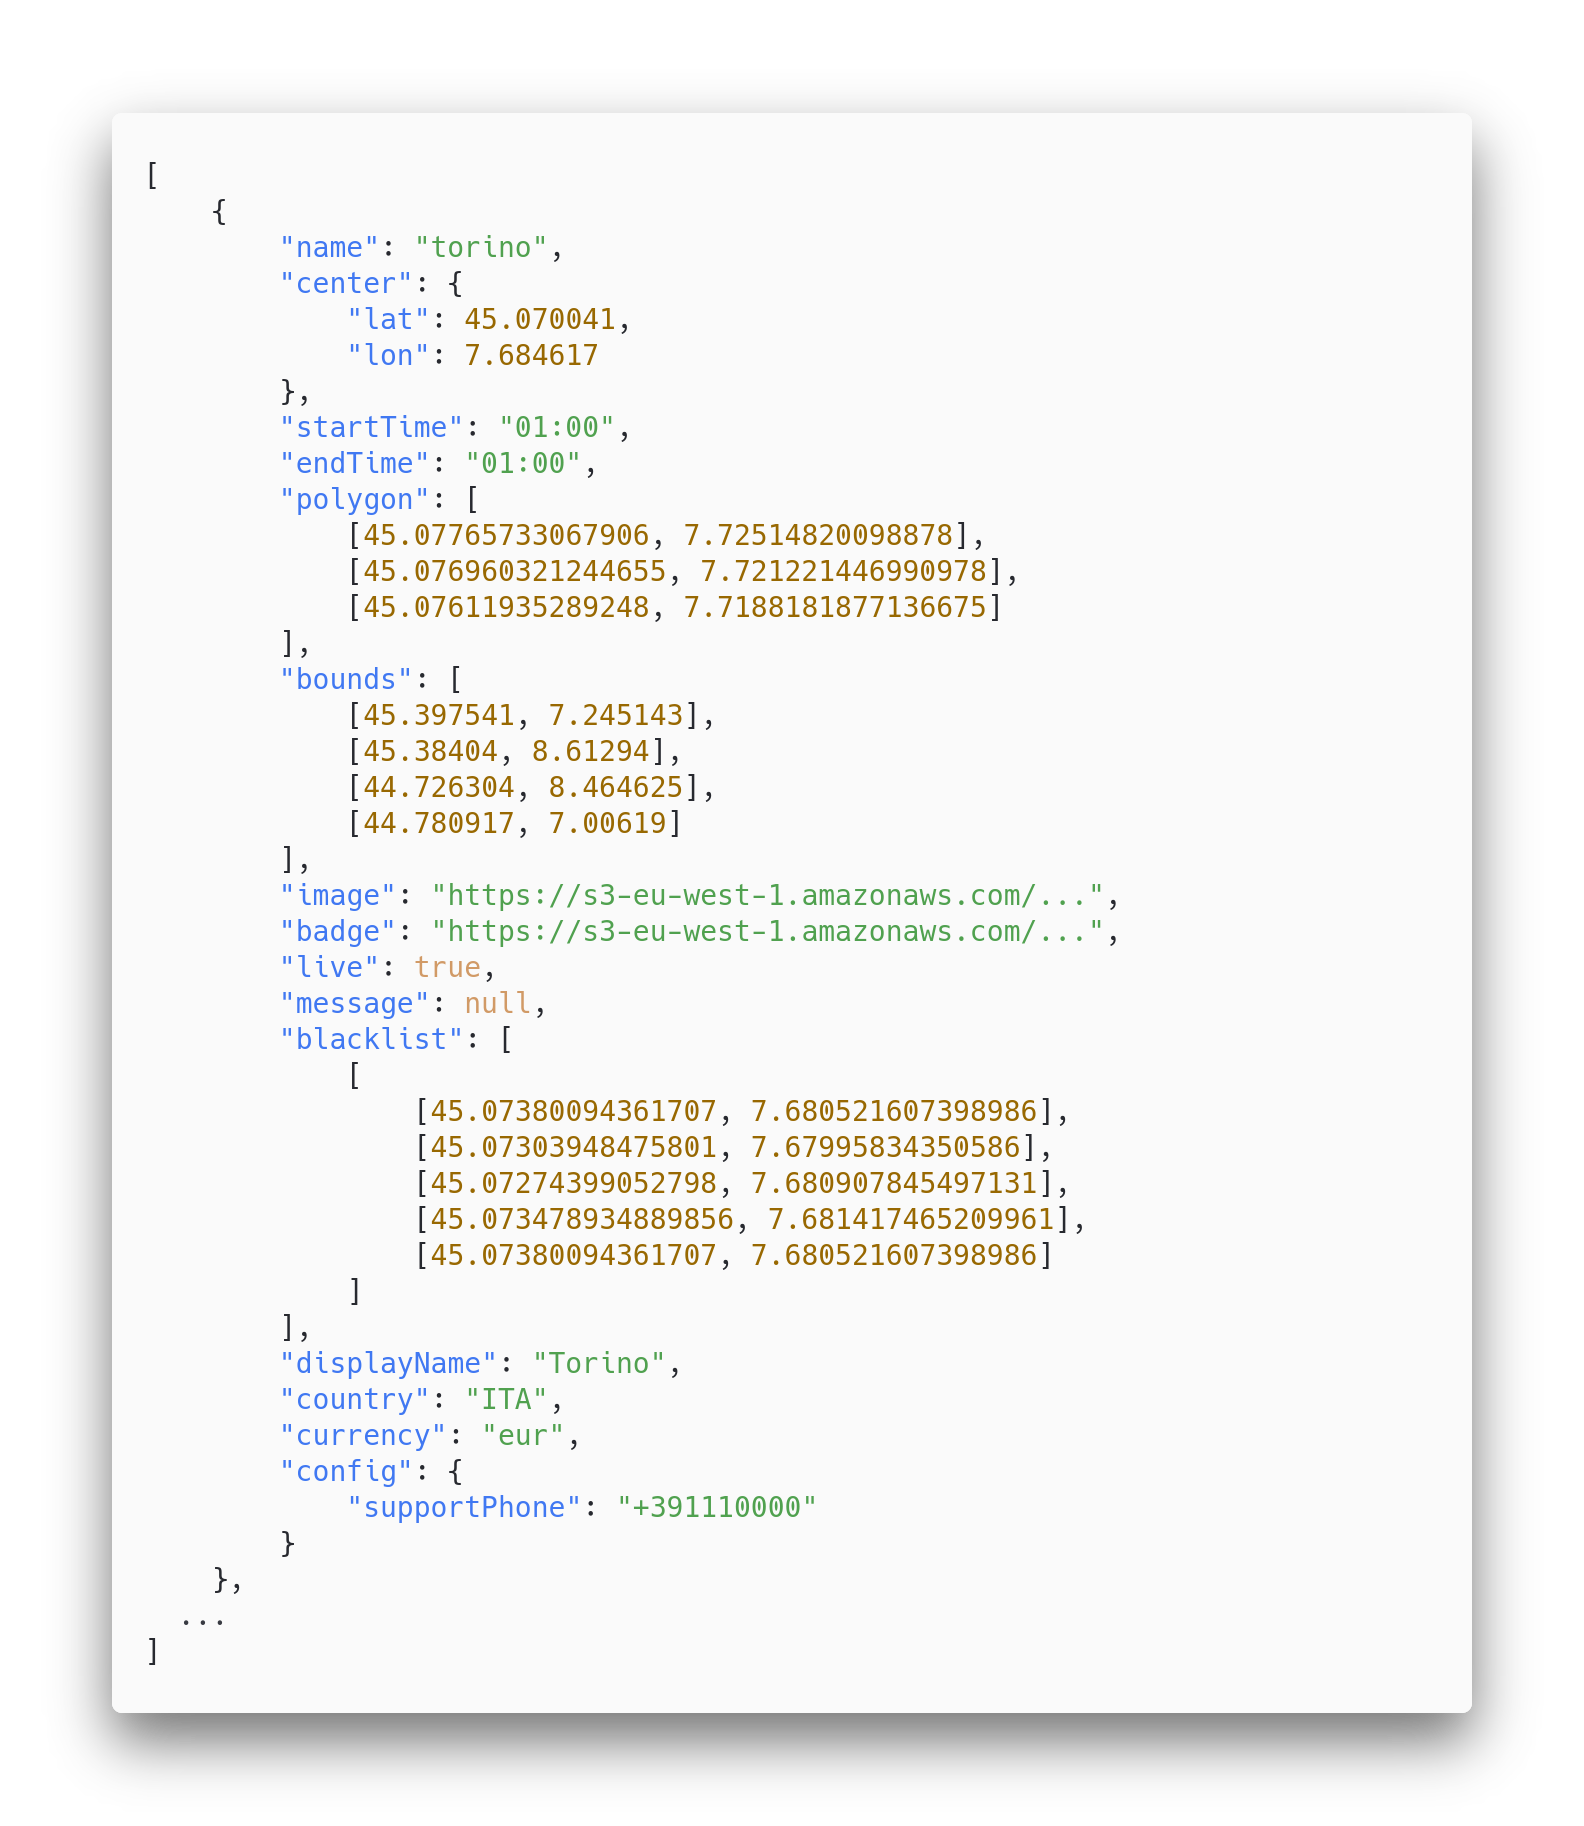
\includegraphics[width=\textwidth]{regionjson.png}
\caption*{Esempio di risposta API regions}
\label{fig:footprint}
\end{figure}


%\begin{minipage}[]{\linewidth}
%\inputminted[bgcolor=white]{json}{region.json}
%\end{minipage}

\subsubsection{API Vehicles}

\textbf{Method:} \texttt{GET} \\
\textbf{Url:} \texttt{https://api.helbiz.com/prod/vehicles?northWest=...\&southEast=...} \\

\begin{table}[h]
\centering
\resizebox{\textwidth}{!}{%
\begin{tabular}{|l|l|l|}
\hline
\rowcolor[HTML]{3166FF} 
{\color[HTML]{FFFFFF} \textbf{Parametro}} & {\color[HTML]{FFFFFF} \textbf{Esempio}} & {\color[HTML]{FFFFFF} \textbf{Descrizione}}                           \\ \hline
northWest                                 & 45,397541,7,245143                      & Coordinate geografiche dell'estremo Nord Ovest dell'area di interesse \\ \hline
southEast                                 & 44,726304,8,464625                      & Coordinate geografiche dell'estremo Sud Est dell'area di interesse    \\ \hline
\end{tabular}%
}
\end{table}

\noindent\textbf{Descrizione:} la richiesta ritorna i veicoli contenuti nell'area di interesse 
corrispondente al rettangolo avente per estremo superiore sinistro il punto specificato dal
parametro northWest e per estremo inferiore destro il punto specificato dal parametro southEast.
Relativamente al singolo veicolo, le informazioni utilizzate ai fini del progetto sono:
\begin{itemize}
\item id: identificatore del veicolo in formato di stringa alfanumerica (esadecimale);
\item lat: latitudine, numero provvisto di parte decimale di lunghezza variabile 
\item lon: longitudine, numero provvisto di parte decimale di lunghezza variabile
\item batteryLevelInMiles: autonomia in miglia della batteria, numero decimale 
\item range: valore risultante dal prodotto tra batteryLevelInMiles e 1000
\item geofence: nome della region di appartenenza
\end{itemize}
Il seguente listato contiene due veicoli di esempio ritornati interrogando il servizio
con le coordinate indicate nella precedente tabella e facenti riferimento alla \emph{region}
che copre la città di Torino.

%\inputminted[bgcolor=lightgray]{json}{vehicles.json}
\begin{figure}[H]
\centering
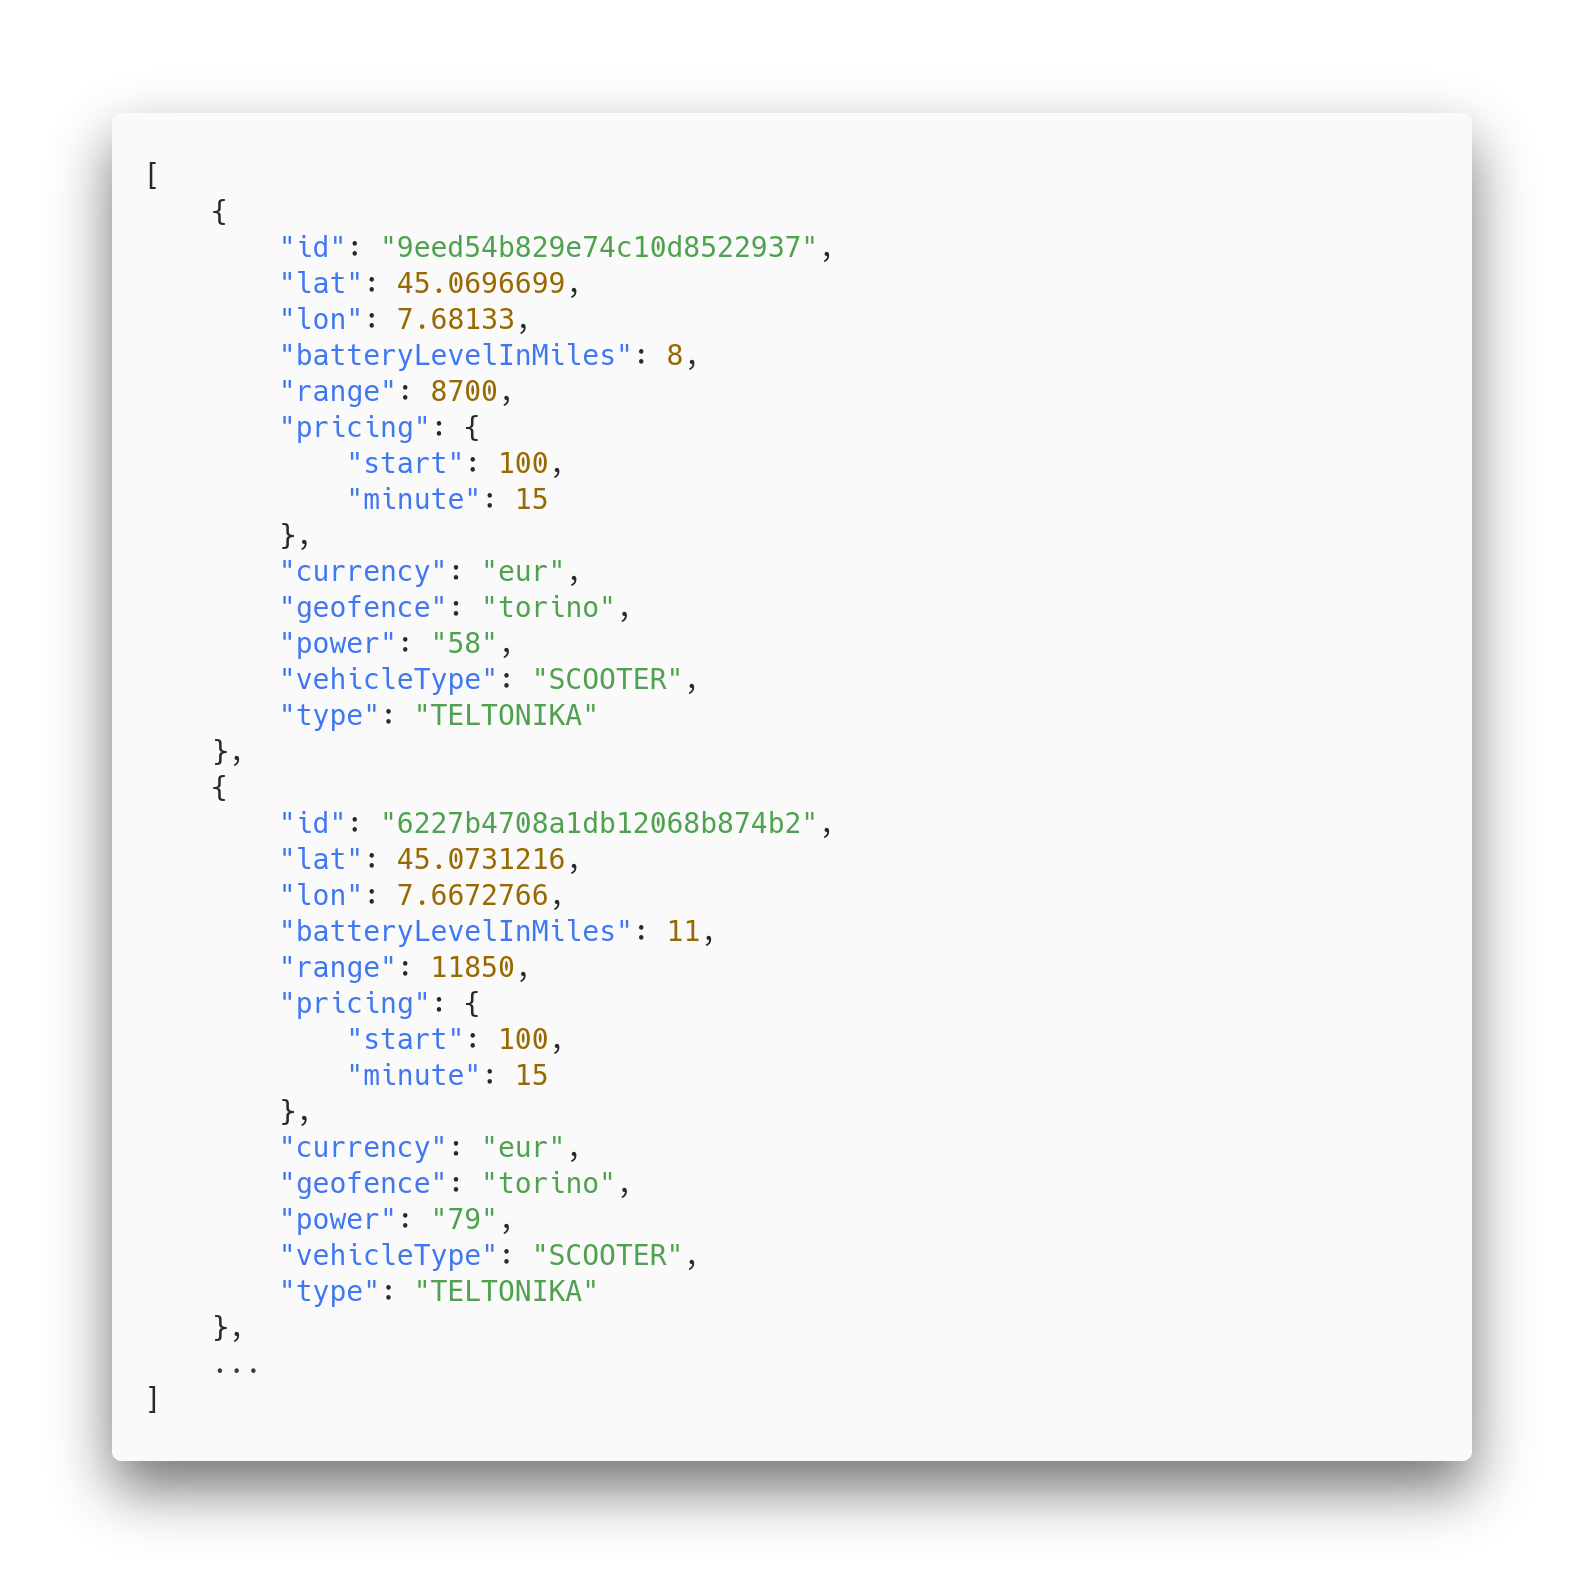
\includegraphics[width=\textwidth]{vehiclesjson.png}
\caption{vehicles.json}
\label{fig:vehiclesjson}
\end{figure}

\subsection{Progettazione concettuale}

A partire dalla API precedentemente descritta è stato scritto un applicativo Java,di cui
verrà fatta descrizione nel seguito, che partendo da una Region e da un intervallo in
minuti interroga ad intervalli regolari il servizio esposto da Helbiz per ottenere le
informazioni sui veicoli presenti in una delimitata area geografica.
In figura~\ref{fig:vehicle_profiling_er} è mostrato lo schema ER che modella le informazioni
relative alle profilazioni. Nella progettazione è stato assunto che ogni istanza
dell'entità Profiling sia univocamente identificata dall'attributo \textit{query\_time} e
dall'attributo \textit{id} dell'entità Vehicle.

\begin{figure}[H]                                                                                                                                                            
\centering                                                                                                                                                                   
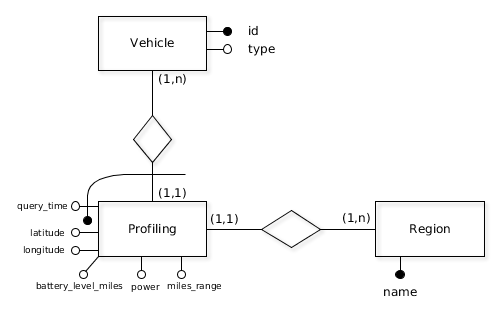
\includegraphics[width=\textwidth]{diagrams/vehicle_profiling_er}                                                                                                                                   
\caption{Diagramma ER Vehicle-Profiling-Region}                                                                                                                                            
\label{fig:vehicle_profiling_er}                                                                                                                                                           
\end{figure}

\subsection{Progettazione logica}

Risultato della progettazione logica sono le seguenti due relazioni:
\begin{itemize}
\item \textit{Vehicles:} contenente tutti dati relativi alla profilazione di un veicolo
appartenente ad una determinata regione in un dato istante di tempo; è presente un
vincolo di integrità referenziale per l'attributo \textit{region\_id} rispetto
all'attributo \textit{id} della relazione \textit{Regions};
\item \textit{Regions:} contenente i nomi delle regioni per le quali esistono delle
profilazioni all'interno della relazione \textit{Vehicles}.
\end{itemize}
In figura~\ref{fig:vehicles_logic_physic} è mostrato lo schema logico ottenuto mediante
l'applicativo MySQL Workbench.

Al fine di semplificare la scrittura dell'applicativo utilizzato per ottenere i dati
dei veicoli dalla sorgente, le entità \textit{Vehicle} e \textit{Vehicle\_profiling} 
sono state rappresentate nella stessa relazione \textit{vehicles}.
Alla relazione \textit{regions} è stata aggiunta una chiave surrogata referenziata
dall'attributo \textit{city\_id} della relazione \textit{vehicles}.

\begin{figure}[H]                                                                                                                                                            
\centering                                                                                                                                                                   
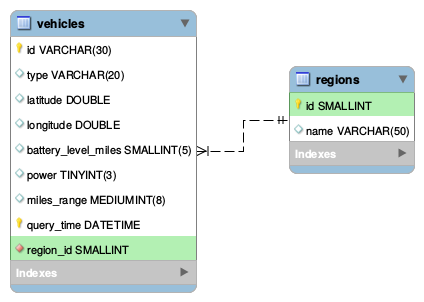
\includegraphics[width=\textwidth]{diagrams/vehicles_logic}                                                                                                                                   
\caption{Schema logico Vehicles}                                                                                                                                            
\label{fig:vehicles_logic_physic}                                                                                                                                                           
\end{figure}

\subsection{Note di utilizzo}

L'applicativo Java scritto per interrogare il servizio descritto sopra è stato attivo h24
per un periodo di un mese nell'interrogazione ad intervalli regolari di 5 minuti dei dati
della region relativa alla città di Torino.

\section{Torinometeo}
Nata nel 2004 come associazione amatoriale di meteo appassionati, Torinometeo oggi è ufficialmente
riconosciuta come associazione culturale con l'obiettivo di porsi come interlocutore privilegiato
nei confronti delle istituzioni locali.

Il progetto principale, oltre a quello della raccolta dei dati dai vari rilevatori in tutto il Piemonte, è
l'esposizione dei dati sotto forma di servizio Open Data. Le singole rilevazioni non sono processate
in maniera tale da poter affermare che in una certa zona del Piemonte ci sia un rovescio o se ci sia
un caldo torrido, ma sono composte dalle misurazioni effettive che un determinato sensore ha rilevato
in una certa data.

\subsection{API REST}
Di seguito procediamo alla documentazione delle due richieste utilizzate

\subsubsection{API Rilevazioni Realtime}
\textbf{Method:} \texttt{GET} \\
\textbf{Url:} \texttt{https://www.torinometeo.org/api/v1/realtime/data} \\

\noindent\textbf{Descrizione:} la richiesta ritorna per ogni rilevatore l'ultima (e ultima soltanto)
rilevazione effettuata. Notasi che ogni sensore ha un proprio \emph{refresh rate} e che questo non viene
dichiarato.

\begin{figure}[H]
\centering
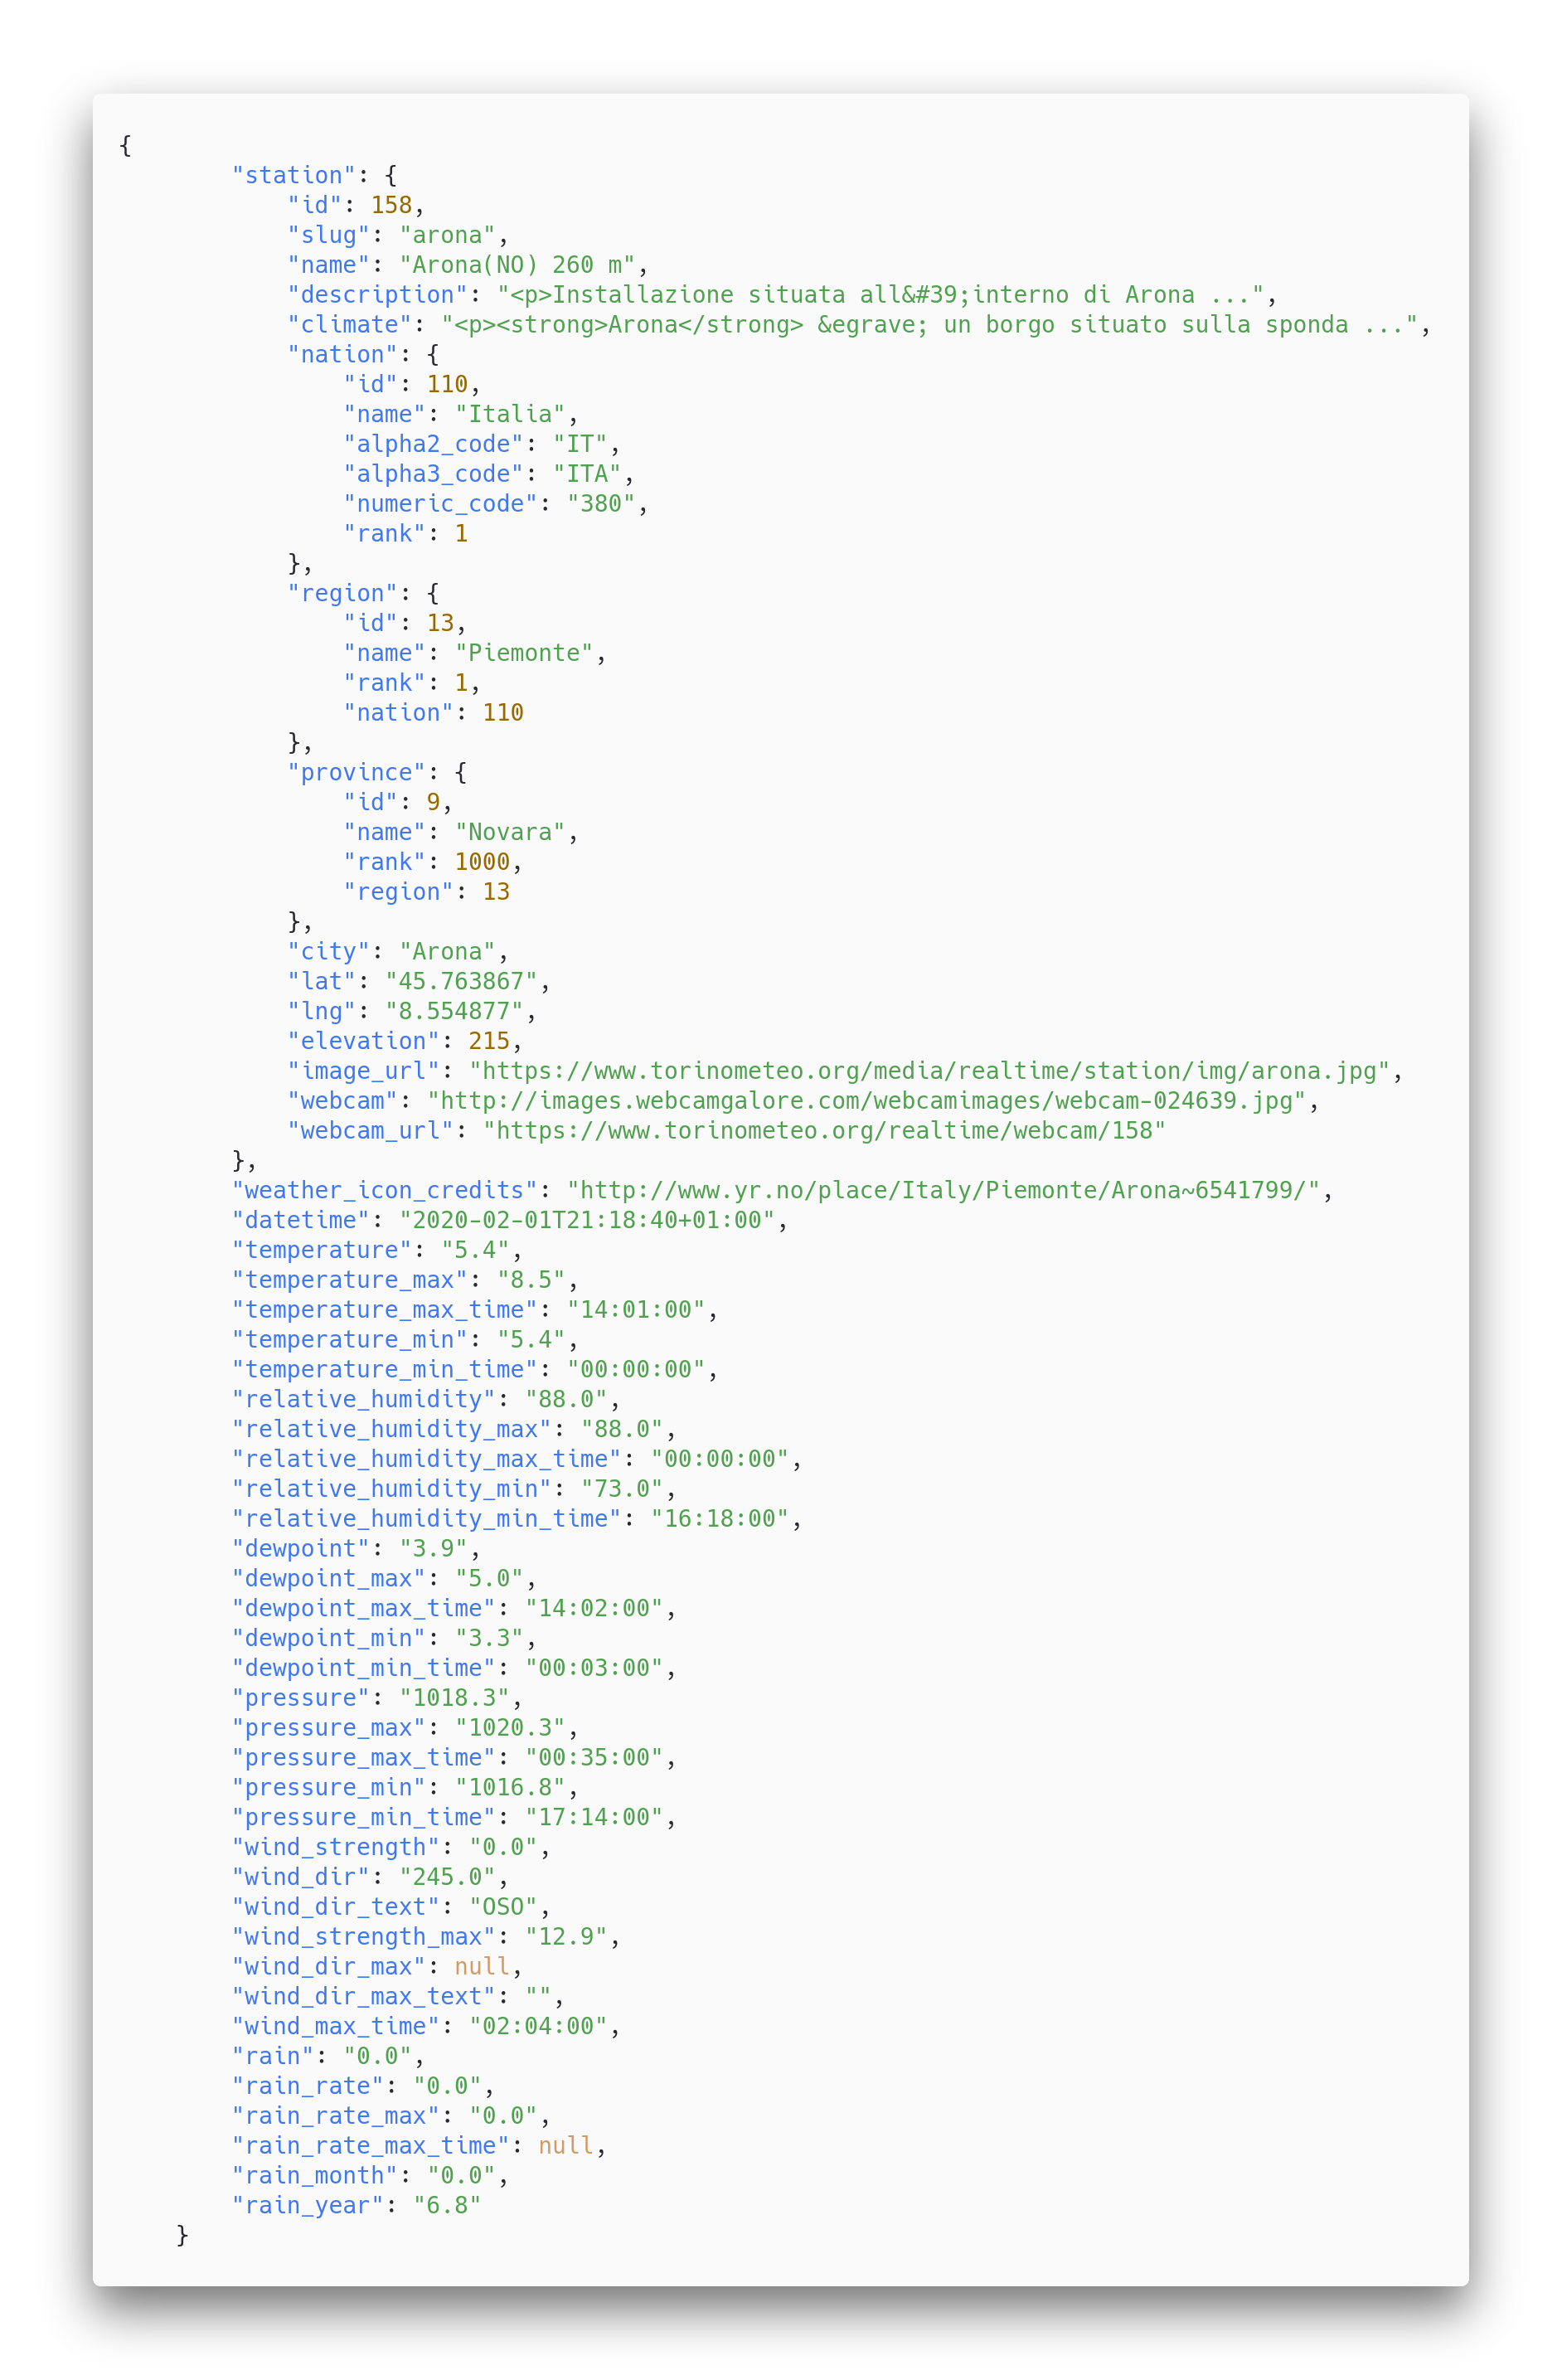
\includegraphics[width=\textwidth]{realtimejson.png}
\caption*{Esempio di risposta realtime}
\label{fig:realtimejson}
\end{figure}


\subsubsection{API Rilevazioni Storiche}
\textbf{Method:} \texttt{GET} \\
\textbf{Url:} \texttt{https://www.torinometeo.org/api/v1/realtime/history/<year>/<month>/<day>} \\

\noindent\textbf{Descrizione:} la richiesta ritorna per ogni rilevatore la rilevazione storica per quella
determinata data.

\begin{table}[h]
\centering
\begin{tabular}{|l|l|l|}
\hline
\rowcolor[HTML]{3166FF} 
{\color[HTML]{FFFFFF} \textbf{Parametro}} & {\color[HTML]{FFFFFF} \textbf{Esempio}} & {\color[HTML]{FFFFFF} \textbf{Descrizione}}                           \\ \hline
year                                 & 2016                      & Anno in formato \texttt{yyyy} \\ \hline
month                                 & 05                      & Mese in formato \texttt{M} o \texttt{MM}    \\ \hline
day                                 & 14                      & Giorno del mese in formato \texttt{d} o \texttt{dd}    \\ \hline
\end{tabular}%

\end{table}


\begin{figure}[H]
\centering
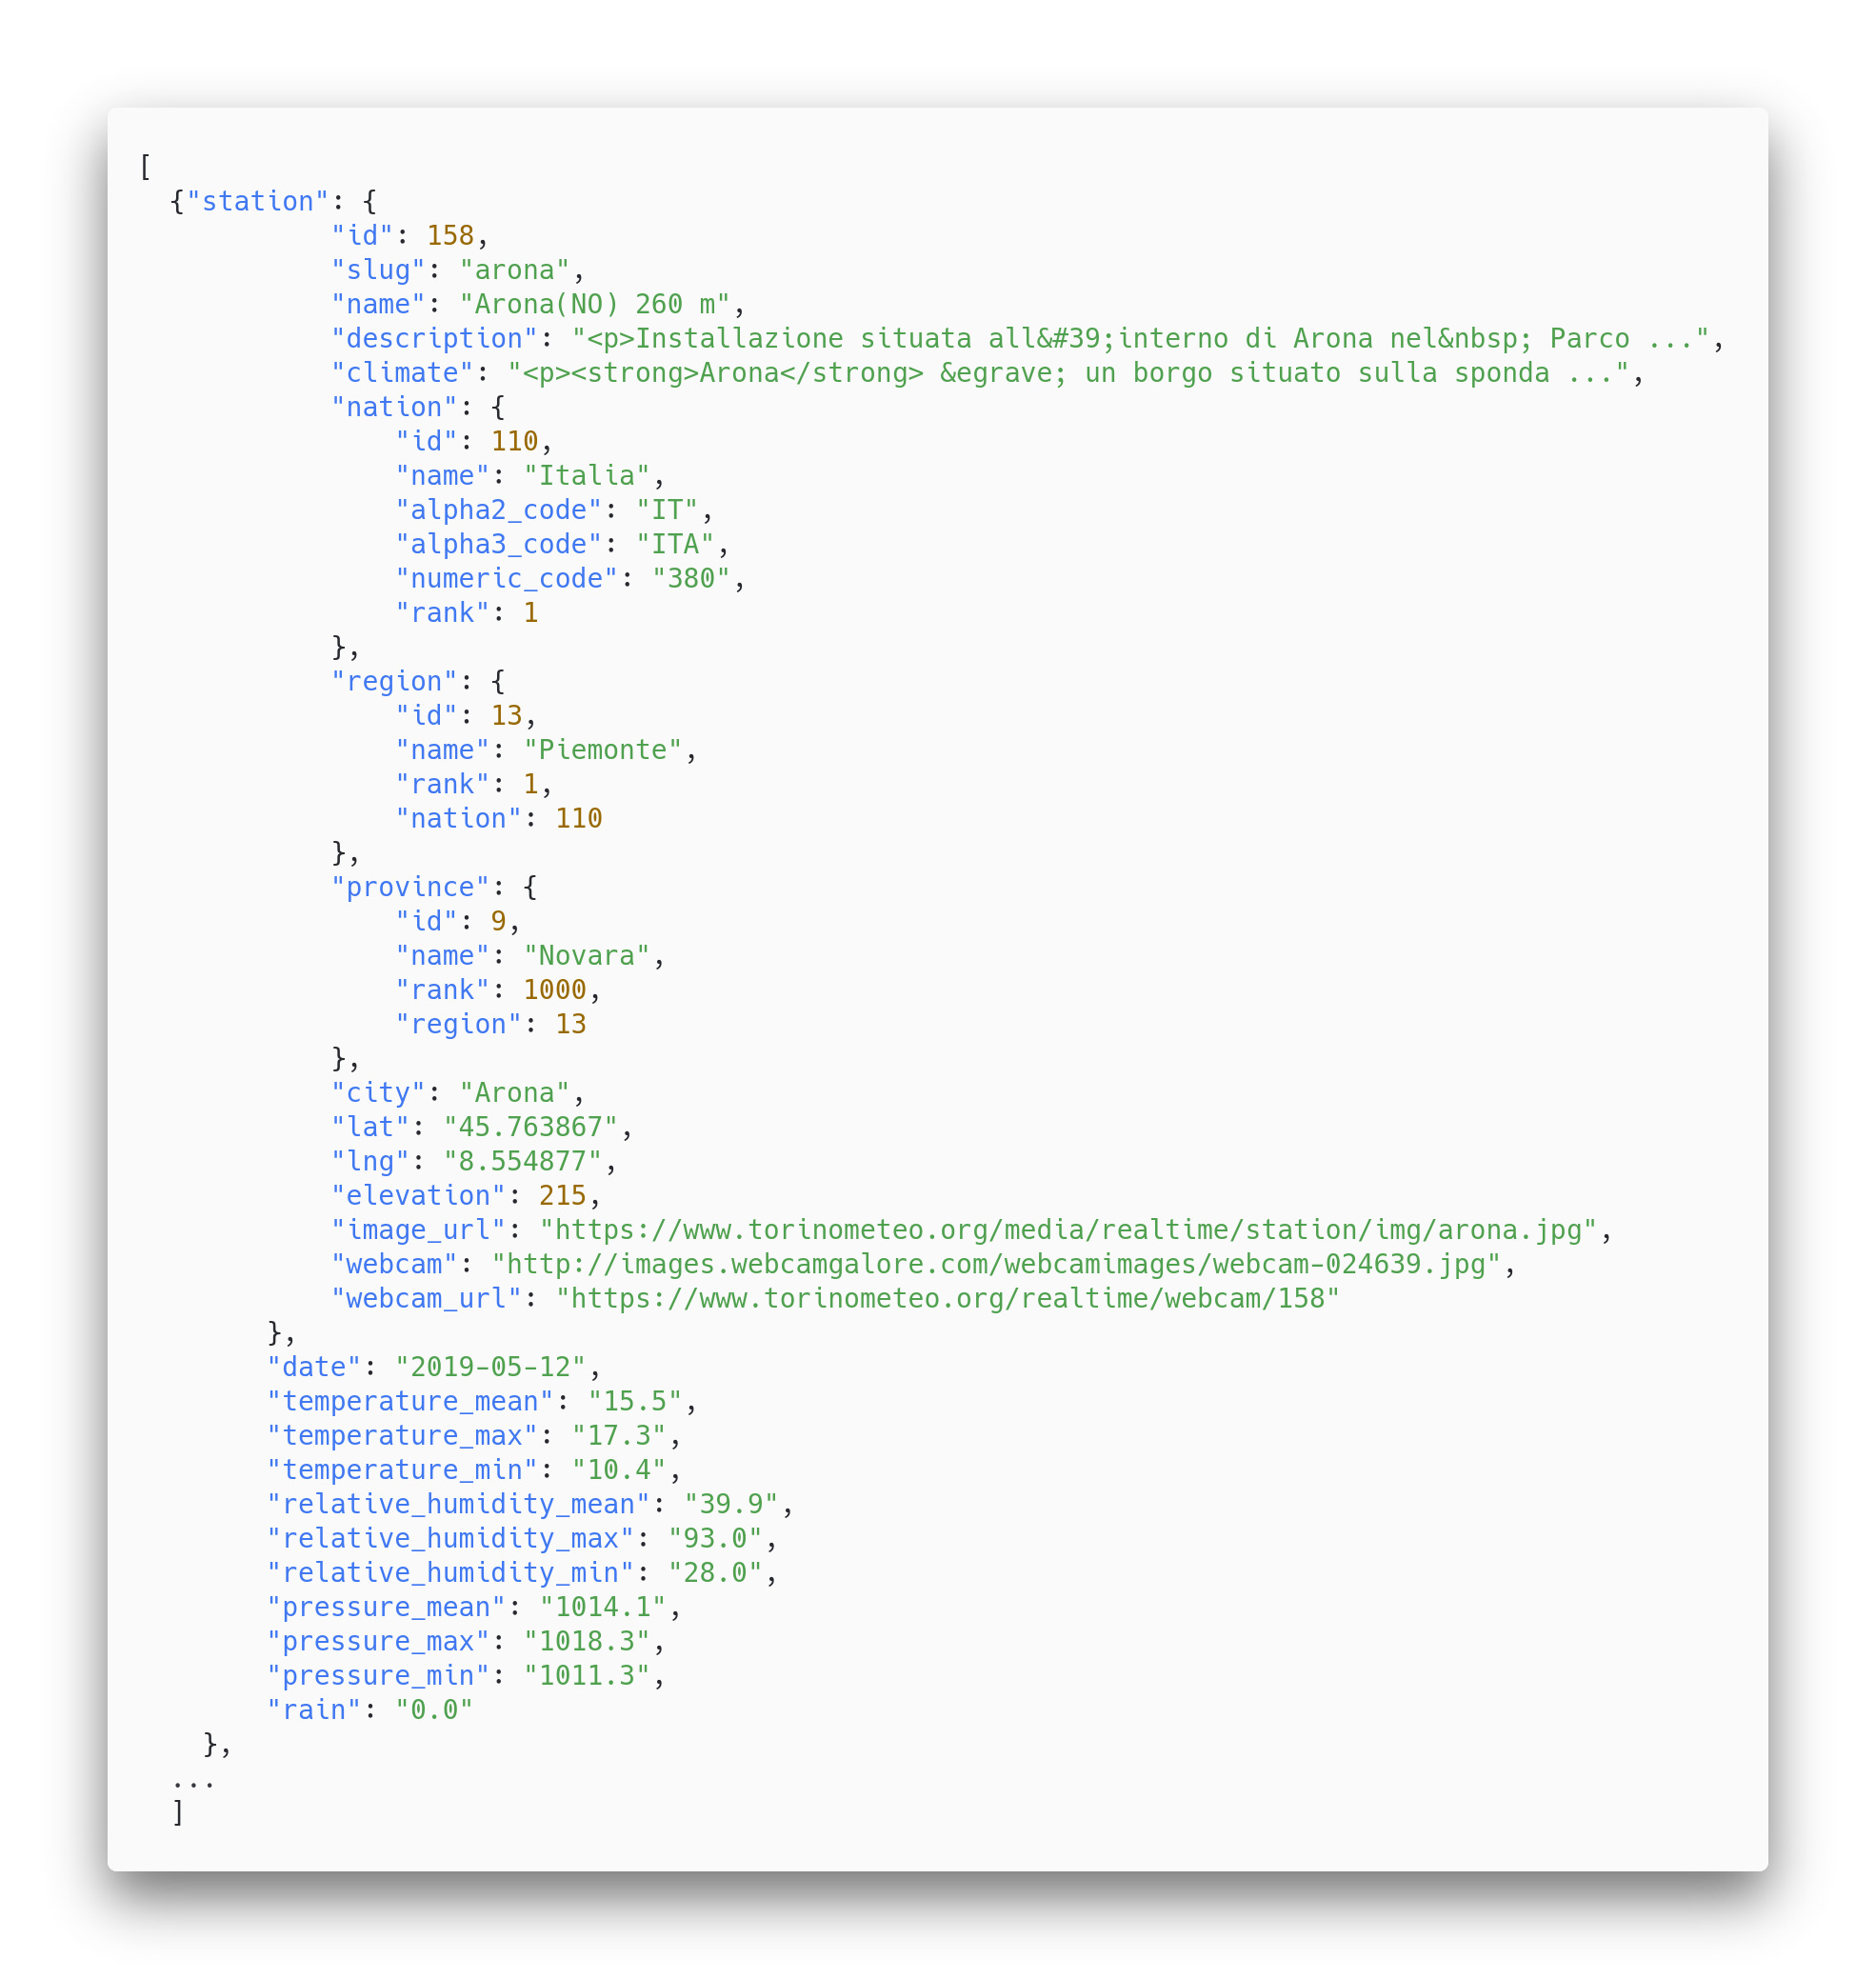
\includegraphics[width=\textwidth]{historicaljson.png}
\caption*{Esempio di risposta di rilevazione storica}
\label{fig:historicaljson}
\end{figure}

\subsection{Progettazione concettuale}

In figura~\ref{fig:weather_detection_er} è mostrato lo schema ER per la sorgente in oggetto.
L'entità \textit{Weather sensor} è univocamente identificata dagli attributi id e detection\_time.

\begin{figure}[H]                                                                                                                                                            
\centering                                                                                                                                                                   
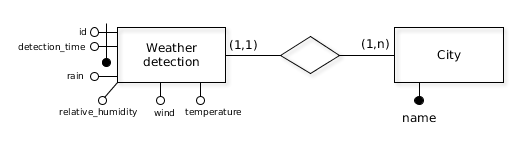
\includegraphics[width=\textwidth]{diagrams/weather_detection_er}                                                                                                                                   
\caption{Diagramma ER Weather sensor-City}                                                                                                                                            
\label{fig:weather_detection_er}                                                                                                                                                           
\end{figure}

\subsection{Progettazione logica}

Si è scelto di creare le seguenti due relazioni:
\begin{itemize}
\item \textit{Weather dectection:} contenente tutti i dati ottenuti interrogando un sensore;
l'attributo è stato posto un vincolo di integrità referenziale sull'attributo
\textit{city\_id} verso la relazione \textit{Cities};
\item \textit{Cities:} contenente i nomi delle città per le quali è presente almeno una
rilevazione nella relazione \textit{Weather detection}.
\end{itemize}
Lo schema logico prodotto è mostrato in figura~\ref{fig:weather_detection_logic}.
La relazione uno a molti tra l'entità \textit{Weather\_sensor} dello schema concettuale e
l'entità \textit{City} è stata trasformata in una relazione uno a uno in quanto, considerato 
a regime il numero di sensori di molto superiore al numero di città osservate, l'aggiunta di
due attributi alla relazione \textit{Cities} atti ad identificare un sensore in essa presente,
avrebbe comportato la presenza di ridondanza nei dati memorizzati.

\begin{figure}[H]                                                                                                                                                            
\centering                                                                                                                                                                   
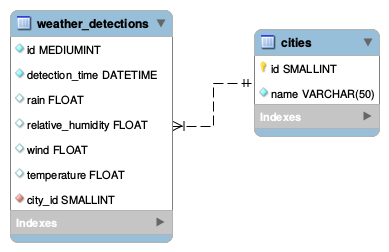
\includegraphics{diagrams/weather_detection_logic}                                                                                                                                   
\caption{Schema logico Weather detections}                                                                                                                                            
\label{fig:weather_detection_logic}                                                                                                                                                           
\end{figure}


\subsection{Note di utilizzo}

Tenuto in considerazione che i dati storici sono su base giornaliera e non riportano la
i dati relativi al vento, la scelta è ricaduta sull'utilizzo della API realtime per la
profilazione oraria delle condizione meteorologiche. La API storica è utilizzata qualora
si riscontri un malfunzionamento di quella realtime.

Similmente a quanto fatto per Helbiz, è stato scritto un applicativo Java allo scopo di
interrogare ogni 5 minuti i sensori di interesse e memorizzarne i dati ottenuti in un
database.


\section{Scioperi}

Per quanto riguarda gli scioperi, è stato utilizzato un dataset rilasciato come Open Data
dal Ministero dei Trasporti della Repubblica Italiana, il quale contiene dati storici
relativi agli scioperi avvenuti o previsti a partire dal 1$^\circ$ Gennaio 2014.

I dati sono messi a disposizione tramite un file CSV che, aggiornato su base giornaliera,
contiene tutti i dati sugli scioperi fino alla data corrente. Vi è inoltre un solo 
endpoint REST, documentato di seguito, che permettono di ricevere una risposta in formato
JSON di quanto contenuto nel file CSV.

\subsection{API REST}

\subsection{API Storico Scioperi}

\textbf{Method:} \texttt{GET} \\
\textbf{Url:} \texttt{http://dati.mit.gov.it/catalog/api/action/\\datastore\_search?resource\_id=6838feb1-1f3d-40dc-845f-d304088a92cd} \\

\noindent\textbf{Descrizione:} la richiesta ritorna la lista degli scioperi a fronte di
un filtraggio opzionale sulla base dei parametri descritti nella seguente tabella.

\begin{table}[H]
\centering
\resizebox{\textwidth}{!}{%
\begin{tabular}{|l|l|l|l|}
\hline
\rowcolor[HTML]{3166FF} 
{\color[HTML]{FFFFFF} \textbf{Parametro}} & {\color[HTML]{FFFFFF} \textbf{Esempio}} & {\color[HTML]{FFFFFF} \textbf{Opzionale}} & {\color[HTML]{FFFFFF} \textbf{Descrizione}}        \\ \hline
q                                         & pubblico                                & Sì                                        & Stringa utilizzata per ricerca testuale tra i dati \\ \hline
limit                                     & 100                                     & Sì                                        & Numero massimo di risultati in risposta            \\ \hline
\end{tabular}%
}
\end{table}

\begin{figure}[H]
\centering
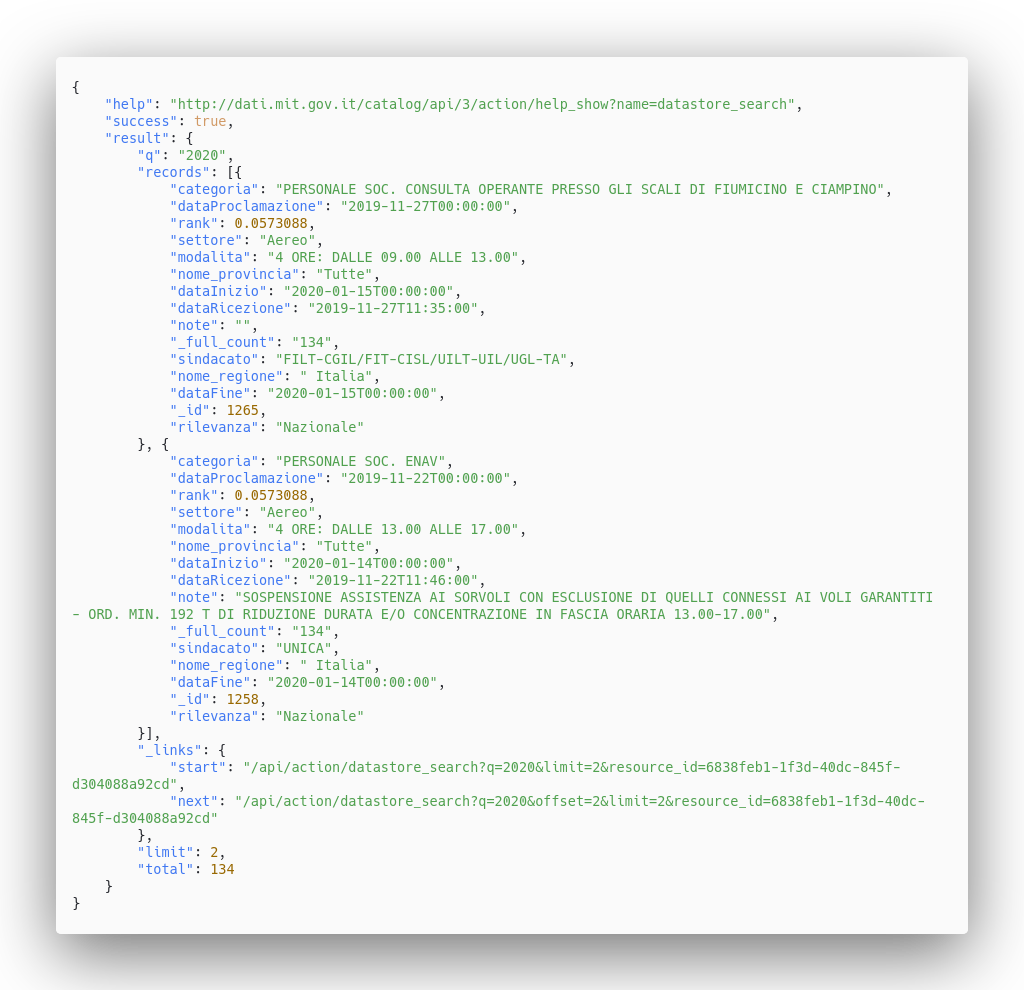
\includegraphics[width=\textwidth]{scioperiJson.png}
\caption*{Esempio di risposta dalla sorgente Scioperi}
\label{fig:historicaljson}
\end{figure}

\subsection{Progettazione concettuale}

In figura~\ref{fig:strikes_er} è presente il diagramma entità relazione per i dati
ottenuti dall'API descritta al punto precedente.
Le istanze dell'entità \textit{Strike} sono identificate univocamente dalla chiave composta
dagli attributi \textit{start\_time}, \textit{end\_time}, \textit{name}, \textit{City} e
\textit{area\_of\_interest}.

\begin{figure}                                                                                                                                                            
\centering                                                                                                                                                                   
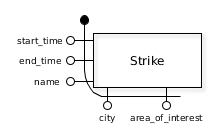
\includegraphics[width=\textwidth/2]{diagrams/strikes_er}                                                                                                                                   
\caption{Diagramma ER Strike-City}                                                                                                                                            
\label{fig:strikes_er}                                                                                                                                                           
\end{figure}

\subsection{Progettazione logica}

Lo schema logico è mostrato in figura~\ref{fig:strikes_logic}.
Presupponendo il numero di scioperi di molto inferiore rispetto al numero di profilazioni
ottenute con le precedenti due sorgenti dati, è stata definita una sola relazione
\textit{Strikes} avente gli stessi attributi dell'entità \textit{Strike} del precedente 
schema ER.

\begin{figure}                                                                                                                                                            
\centering                                                                                                                                                                   
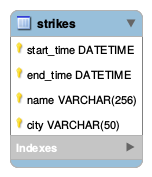
\includegraphics{diagrams/strikes_logic}                                                                                                                                   
\caption{Schema logico Strikes}                                                                                                                                            
\label{fig:strikes_logic}                                                                                                                                                           
\end{figure}

\subsection{Note di utilizzo}

Nonostante il dataset riporti, oltre agli scioperi avvenuti, quelli programmati,
considerato che i dati in oggetto sono da utilizzarsi solo a corredo dei dati
ottenuti dalle rilevazioni delle precedenti due sorgenti, si è scelto di filtrare
tra i risultati restituiti dalla API, i soli scioperi risalenti ad almeno due
giorni dalla data della richiesta e pertanto già avvenuti.

Si segnala inoltre come gli attributi \textit{data\_inizio} e \textit{data\_fine} 
riportino sempre lo stesso valore mentre l'intervallo di validità dello sciopero
sia esplicitato in maniera eterogenea tra i risultati dall'attributo
\textit{modalità}.

Come per le altre due sorgenti, è stato scritto un applicativo Java che si occupa
di:
\begin{itemize}
\item reperire al primo avvio tutti i dati relativi agli scioperi avvenuti
nell'anno in corso fino a due giorni dalla data corrente e salvarli su di
un'apposita base dati;
\item aggiornare giornalmente la base date con gli scioperi avvenuti nei
precedenti due giorni.
\end{itemize}
